% Agern: Getting Started. Build with scripts/manual.sh (screenshots, checks and the PDF), which runs
%   latexmk -pdf -outdir=../../build/manual/tex -usepretex='\def\agernversion{<version>}' manual.tex
% in this directory. One file per chapter in chapters/.
\providecommand{\agernversion}{development build}
\documentclass[11pt,a4paper,oneside,openany]{report}
% Packages and macros of the manual. Only packages from TeX Live's latex-base, latex-recommended,
% latex-extra, fonts-recommended and pictures collections (see README.md, "Manual").
\usepackage[utf8]{inputenc}
\usepackage[T1]{fontenc}
\usepackage{lmodern}
\usepackage{textcomp}
\usepackage{amssymb}
\usepackage[a4paper,margin=2.3cm,headheight=14pt]{geometry}
\usepackage{graphicx}
\usepackage[table]{xcolor}
\usepackage{microtype}
\usepackage{booktabs}
\usepackage{tabularx}
\usepackage{longtable}
\usepackage{array}
\usepackage[shortlabels]{enumitem}
\usepackage{caption}
\usepackage{listings}
\usepackage{tikz}
\usetikzlibrary{arrows.meta,positioning,fit,calc}
\usepackage[most]{tcolorbox}
\usepackage{fancyhdr}
\usepackage{makeidx}
\usepackage{url}
\usepackage[colorlinks=true,linkcolor=agernlink,urlcolor=agernlink,citecolor=agernlink,
  bookmarksnumbered=true,pdfusetitle=false]{hyperref}
\usepackage{bookmark}

\makeindex

% ---- colours (the app's amber accent on paper)
\definecolor{agernamber}{HTML}{C8761A}
\definecolor{agernlink}{HTML}{1F5F99}
\definecolor{agernink}{HTML}{1F2421}
\definecolor{notebg}{HTML}{EEF4FA}
\definecolor{warnbg}{HTML}{FDF1E3}
\definecolor{codebg}{HTML}{F5F5F2}

\hypersetup{
  pdftitle={Agern: Getting Started},
  pdfauthor={Egernet},
  pdfsubject={Getting-started manual for Agern, version \agernversion},
  pdfkeywords={Agern, software factory, Claude, GitHub},
}

% ---- layout
\setlength{\parindent}{0pt}
\setlength{\parskip}{0.55em plus 0.2em}
\setlength{\emergencystretch}{3em}
\setlist{itemsep=0.25em,topsep=0.4em}
\setlist[enumerate,1]{label=\textbf{\arabic*.},leftmargin=2em}
\captionsetup{font=small,labelfont=bf,margin=1em}
\captionsetup[figure]{skip=6pt}
\renewcommand{\arraystretch}{1.25}
\pagestyle{fancy}
\fancyhf{}
\fancyhead[L]{\small\nouppercase{\leftmark}}
\fancyhead[R]{\small Agern \agernversion}
\fancyfoot[C]{\small\thepage}
\renewcommand{\headrulewidth}{0.3pt}
\fancypagestyle{plain}{\fancyhf{}\fancyfoot[C]{\small\thepage}\renewcommand{\headrulewidth}{0pt}}

% ---- screenshots: every UI image of the manual goes through these two macros, one call per line,
% label last (scripts/manual.sh checks that each label is referenced and each file was produced):
%   \screenshot[<width>]{<file without .png>}{<caption>}{<label>}   -> figure with \label{fig:<label>}
%   \phoneshot[<width>]{<file without .png>}{<caption>}{<label>}    -> the same, narrow (390 px phone shots)
% The files come from build/manual/screenshots/ (web/scripts/screenshots.mjs).
\graphicspath{{../../build/manual/screenshots/}}
\newcommand{\screenshot}[4][\linewidth]{%
  \begin{figure}[htbp]
    \centering
    \setlength{\fboxsep}{0pt}\setlength{\fboxrule}{0.4pt}%
    \fcolorbox{black!30}{white}{\includegraphics[width=\dimexpr#1-0.8pt\relax,height=0.78\textheight,keepaspectratio]{#2}}
    \caption{#3}
    \label{fig:#4}
  \end{figure}}
\newcommand{\phoneshot}[4][0.40\linewidth]{%
  \begin{figure}[htbp]
    \centering
    \setlength{\fboxsep}{0pt}\setlength{\fboxrule}{0.4pt}%
    \fcolorbox{black!30}{white}{\includegraphics[width=\dimexpr#1-0.8pt\relax,height=0.78\textheight,keepaspectratio]{#2}}
    \caption{#3}
    \label{fig:#4}
  \end{figure}}

% ---- text markup
% \term{run}: a glossary term where it is introduced (italic, indexed). \term[index entry]{text}.
\newcommand{\term}[2][]{\emph{#2}\if\relax\detokenize{#1}\relax\index{#2}\else\index{#1}\fi}
% \ui{Start run}: a label of a button, field or page in the web UI.
\newcommand{\ui}[1]{\textsf{\textbf{#1}}}
% \cmd{sudo agern doctor}, \envvar{FACTORY_PUBLIC_URL}: commands and variables (underscores allowed).
\newcommand{\cmd}[1]{\texttt{\detokenize{#1}}}
% (\ttraw is robust, so the index file gets \ttraw{NAME} rather than an expanded name.)
\DeclareRobustCommand{\ttraw}[1]{\texttt{\detokenize{#1}}}
\newcommand{\envvar}[1]{\ttraw{#1}\index{#1@\ttraw{#1}}}
\newcommand{\file}[1]{\path{#1}}
% \msg{...}: a message exactly as Agern shows it.
\newcommand{\msg}[1]{\textsf{``#1''}}
% Links into the repository's reference docs.
\newcommand{\repodoc}[2]{\href{https://github.com/Egernet-CS/agern/blob/main/docs/#1}{#2}}

% ---- boxes
\newtcolorbox{note}[1][Note]{enhanced,breakable,colback=notebg,colframe=agernlink,boxrule=0.4pt,
  left=6pt,right=6pt,top=4pt,bottom=4pt,fonttitle=\bfseries\small,title=#1,arc=2pt}
\newtcolorbox{warning}[1][Warning]{enhanced,breakable,colback=warnbg,colframe=agernamber,boxrule=0.6pt,
  left=6pt,right=6pt,top=4pt,bottom=4pt,fonttitle=\bfseries\small,title=#1,arc=2pt}

% ---- code
\lstdefinestyle{sh}{language=bash,basicstyle=\ttfamily\small,columns=fullflexible,keepspaces=true,
  upquote=true,breaklines=true,breakatwhitespace=false,showstringspaces=false,backgroundcolor=\color{codebg},
  frame=single,rulecolor=\color{black!15},framesep=4pt,xleftmargin=4pt,xrightmargin=4pt,
  commentstyle=\color{black!55},
  breakindent=2em,aboveskip=0.6em,belowskip=0.6em}
\lstdefinestyle{conf}{style=sh,language={}}
\lstset{style=sh}

% ---- "What you have now" ends every chapter.
\newcommand{\whatyouhave}{\section*{What you have now}\addcontentsline{toc}{section}{What you have now}}

% Characters pdfLaTeX's utf8 does not map by itself.
\DeclareUnicodeCharacter{2192}{\ensuremath{\rightarrow}}
\DeclareUnicodeCharacter{2026}{\ldots}
\DeclareUnicodeCharacter{00B7}{\textperiodcentered}
\DeclareUnicodeCharacter{2713}{\ensuremath{\checkmark}}
\DeclareUnicodeCharacter{25B6}{\ensuremath{\blacktriangleright}}


\begin{document}
\pdfbookmark[0]{Title}{title}
\begin{titlepage}
  \centering
  \vspace*{3.5cm}
  \includegraphics[width=4.2cm]{logo}\par
  \vspace{1.2cm}
  {\fontsize{34}{40}\selectfont\bfseries Agern: Getting Started\par}
  \vspace{0.6cm}
  {\Large Install Agern, set it up and put Claude agents to work on your GitHub issues\par}
  \vspace{2.2cm}
  {\large Agern \agernversion\par}
  \vspace{0.3cm}
  {\large Built \today\par}
  \vfill
  {\small Agern is a self-hosted software factory by Egernet. ``Agern'' is Danish for acorn.\par
  This manual explains and links; the reference is
  \href{https://github.com/Egernet-CS/agern/blob/main/docs/ARCHITECTURE.md}{\texttt{docs/ARCHITECTURE.md}}.\par}
\end{titlepage}

\pdfbookmark[0]{Contents}{contents}
\tableofcontents

\chapter*{How to read this manual}
\addcontentsline{toc}{chapter}{How to read this manual}
\markboth{How to read this manual}{}
This manual is a guided path. Read it from start to finish and you will have installed Agern on a
Linux server, set it up, connected your accounts, and taken a GitHub issue all the way to a merged
pull request. It assumes that you know GitHub and a Linux shell, and nothing about Agern or
Claude Code.

Every chapter starts with what you want to achieve, walks you through numbered steps with a
screenshot of what you should see, and ends with \emph{What you have now} and where to go next.

\begin{itemize}
  \item \textbf{Part~\ref{part:setup}, Set up Agern} (chapters~\ref{ch:what}--\ref{ch:sandboxes}): what Agern
    is, installing it on Debian or Ubuntu, configuring it, and connecting your GitHub and Claude accounts.
  \item \textbf{Part~\ref{part:use}, Use Agern} (chapters~\ref{ch:project}--\ref{ch:watch}): projects, the
    project's chat agent, pipeline runs, releases and keeping an eye on the agents.
  \item \textbf{Part~\ref{part:run}, Keep Agern running} (chapters~\ref{ch:upgrade} and~\ref{ch:backup}):
    upgrades, backups, logs and troubleshooting.
\end{itemize}

Words in \emph{italics} where they first appear are Agern terms; they are explained in the
glossary (appendix~\ref{app:glossary}) and listed in the index. Labels in the web UI are set like
\ui{Start run}, commands like \cmd{sudo agern doctor}. The screenshots show Agern's demo data: the
users alice, bob, carl and dora and demo repositories such as \texttt{web-shop}. Host names such as
\texttt{agern.example.com}, the network \texttt{192.0.2.0/24}, the organization \texttt{your-org} and
tokens such as \texttt{ghp\_\ldots} are placeholders for your own values.

The reference documentation lives in the repository and is linked where it matters:
\repodoc{ARCHITECTURE.md}{\texttt{docs/ARCHITECTURE.md}} (how everything works, every setting),
\repodoc{INSTALL-LINUX.md}{\texttt{docs/INSTALL-LINUX.md}} (the installation in depth) and
\repodoc{SANDBOXES.md}{\texttt{docs/SANDBOXES.md}} (sandboxes for project authors).

\part{Set up Agern}\label{part:setup}
\chapter{What Agern is}\label{ch:what}

\emph{You want to know what Agern does and what you need before you install it.} This chapter
gives you the idea in two pages and the shopping list.

\section{The idea}\label{sec:idea}

Agern is a web application that you run on your own server. It puts Claude agents to work on
the issues of your GitHub organization, and the organization is the source of truth:

\begin{itemize}
  \item \textbf{Repositories are projects.} Every repository of the organization that your own
    GitHub token can read appears as a \term{project} in Agern. A \term{workspace project} is a
    repository that brings several repositories together; its members are worked on side by side.
  \item \textbf{Every project has a chat agent.} The project page has a terminal-like
    \term{chat} with an \term{agent}: a Claude Code process working in a checkout of the
    repository. You ask it about the code, attach screenshots, or let it write an issue for you
    (chapter~\ref{ch:chat}). Each conversation with an agent, and each pipeline stage, is a
    \term{session}.
  \item \textbf{Issues are the work.} An \term{issue} on GitHub is a task. Anyone who can see the
    project can hand an issue to the pipeline.
  \item \textbf{The pipeline turns an issue into a merged pull request.} A pipeline \term{run}
    takes one issue through fixed \term[stage]{stages}, each done by its own agent
    (figure~\ref{fig:pipeline}). A spec-writer writes a specification. A builder implements it on
    a branch and opens a pull request. Four \term[reviewer]{reviewers} (security, UX, UI design
    and code quality) inspect the change in parallel, each with the \term{verdict} PASS or
    CHANGES. Changes send the work back to the same builder for a \term[round]{fix round}. When
    all four pass, an \term{approver} makes the final call: it approves, and Agern squash-merges
    the pull request and closes the issue, or it escalates, and the run \term[needs human]{needs a human}: you.
  \item \textbf{Releases bundle issues.} A \term{release} is a plan of several issues that
    Agern builds one after another on a branch of its own and merges in one pull request
    (chapter~\ref{ch:releases}).
\end{itemize}

The order of the stages is decided by Agern's server, not by a model: a run always goes the same
way. Which Claude model does which job is a setting of yours (section~\ref{sec:models}).

\begin{figure}[htbp]
  \centering
  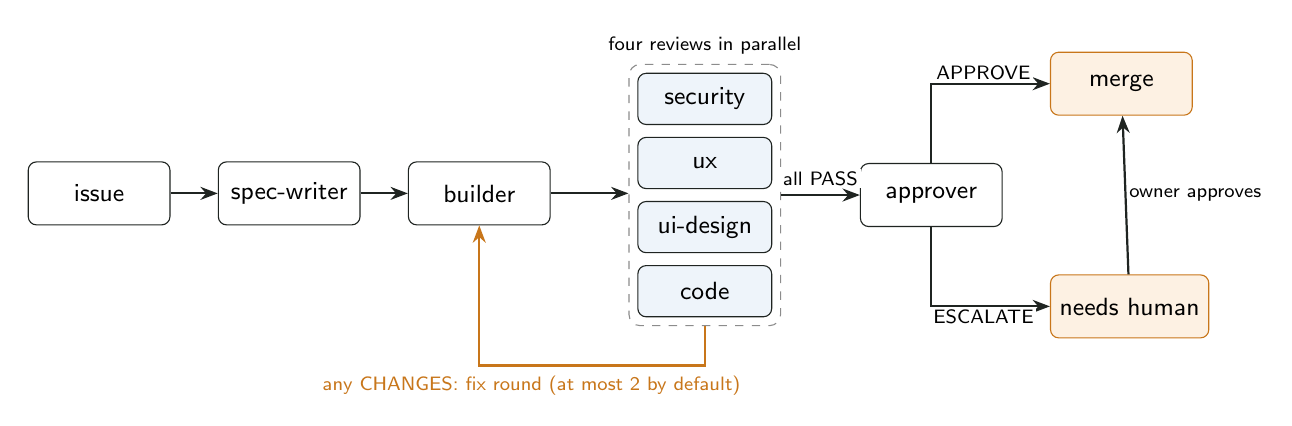
\begin{tikzpicture}[
      font=\sffamily\small,
      node distance=5mm and 6mm,
      stage/.style={draw=agernink,rounded corners=3pt,fill=white,minimum width=18mm,minimum height=8mm,align=center},
      review/.style={stage,minimum width=17mm,minimum height=6.5mm,fill=notebg},
      outcome/.style={stage,draw=agernamber,fill=warnbg},
      arr/.style={-{Stealth[length=2.2mm]},thick,draw=agernink},
      lab/.style={font=\sffamily\scriptsize,fill=white,inner sep=1pt}]
    \node[stage] (issue) {issue};
    \node[stage,right=of issue] (spec) {spec-writer};
    \node[stage,right=of spec] (build) {builder};
    \node[review,right=11mm of build,yshift=12mm] (sec) {security};
    \node[review,below=1.5mm of sec] (ux) {ux};
    \node[review,below=1.5mm of ux] (ui) {ui-design};
    \node[review,below=1.5mm of ui] (code) {code};
    \node[draw=black!45,dashed,rounded corners=4pt,inner sep=3pt,fit=(sec)(code)] (four) {};
    \node[font=\sffamily\scriptsize,above=0mm of four] {four reviews in parallel};
    \node[stage,right=10mm of four] (appr) {approver};
    \node[outcome,above right=6mm and 6mm of appr] (merge) {merge};
    \node[outcome,below right=6mm and 6mm of appr] (human) {needs human};
    \draw[arr] (issue) -- (spec);
    \draw[arr] (spec) -- (build);
    \draw[arr] (build) -- (build -| four.west);
    \draw[arr] (four.east |- appr) -- node[lab,above=2pt] {all PASS} (appr);
    \draw[arr] (appr) |- node[lab,pos=0.72,above] {APPROVE} (merge);
    \draw[arr] (appr) |- node[lab,pos=0.72,below] {ESCALATE} (human);
    \draw[arr] (human) -- node[lab,right] {owner approves} (merge);
    \draw[arr,draw=agernamber] (four.south) -- ++(0,-5mm) -| (build.south);
    \node[lab,text=agernamber] at ($(four.south)+(-22mm,-7.5mm)$) {any CHANGES: fix round (at most 2 by default)};
  \end{tikzpicture}
  \caption{The pipeline of a run. Reviews that ask for changes send the work back to the builder;
    when the approver escalates, the run waits for its owner.}
  \label{fig:pipeline}
\end{figure}

\subsection*{Whose account pays}

Agern has no Claude account and no GitHub account of its own. Each person registers their own
Claude credential and their own GitHub token in Agern's settings (chapter~\ref{ch:accounts}). An
agent always runs with the credentials of the person who started it, its \term{owner}. Nobody,
not even an \term{admin}, can make an agent run on someone else's account; admins may stop or
cancel agents, never drive them. Everybody who can read a repository can watch its agents as an
\term{observer}, read-only.

\section{What you need}\label{sec:needs}

\begin{enumerate}
  \item \textbf{A Linux server} with Debian~13 (recommended) or Ubuntu~24.04 LTS and systemd, a
    fixed address and a name on your network. Agern itself is light; the agents are not, because
    each one clones repositories and runs builds and tests. From
    \repodoc{INSTALL-LINUX.md\#1-the-machine}{\texttt{INSTALL-LINUX.md}, section~1}:

    \begin{center}
    \begin{tabular}{@{}lll@{}}
      \toprule
      & Minimum & Recommended (a few people, several runs at once)\\
      \midrule
      vCPU & 4 & 8\\
      RAM & 8 GB & 16--32 GB\\
      Disk & 64 GB & 128 GB or more\\
      \bottomrule
    \end{tabular}
    \end{center}
  \item \textbf{A GitHub organization} whose repositories become the projects, for example
    \texttt{your-org}.
  \item \textbf{A GitHub token} for each person: a personal access token that can read and write
    the organization's repositories (section~\ref{sec:github-token}).
  \item \textbf{A Claude credential} for each person: an OAuth token from \cmd{claude setup-token}
    (with a Claude subscription) or an Anthropic API key (section~\ref{sec:claude-credential}).
\end{enumerate}

\begin{warning}[Security boundary: use a dedicated machine]
All agents run as one operating-system user, \texttt{agern}, with Claude Code's permission checks
bypassed. Agents of different people can therefore read each other's work and anything else
that user can read on the machine. Run Agern on a dedicated machine or virtual machine that holds
nothing else of value, keep it on a trusted network, and never add the \texttt{agern} user to
\texttt{sudo} or \texttt{docker}. Details:
\repodoc{INSTALL-LINUX.md\#11-security-boundary}{\texttt{INSTALL-LINUX.md}, section~11}.
\end{warning}

\whatyouhave
You know the parts of Agern (projects, chat agents, issues, runs and releases) and you have a
server, an organization and the two credentials ready, or know where to get them. Next,
install Agern on the server: chapter~\ref{ch:install}.

\chapter{Install}\label{ch:install}

\emph{You want Agern running on your server and to sign in to it as its first admin.} You install
the Debian package, give Agern a database and a minimal configuration, install the tools the
agents use, and sign in with two-factor authentication. Allow about half an hour.

Do all of this on the server, over SSH, as a user that may use \cmd{sudo}. The
\repodoc{INSTALL-LINUX.md}{installation guide} has the same steps with more background, and a
section on creating the virtual machine on Proxmox.

\section{Install PostgreSQL}\label{sec:postgres}

Agern keeps its data in PostgreSQL~15 or newer, installed from the distribution (Debian~13 ships
17, Ubuntu~24.04 ships 16).

\begin{enumerate}
  \item Update the package lists and install PostgreSQL:
\begin{lstlisting}
sudo apt update
sudo apt install postgresql
\end{lstlisting}
\end{enumerate}

\section{Download, verify and install the package}\label{sec:install-deb}

Every release of Agern on GitHub carries the package \texttt{agern\_<version>\_all.deb} and a file
\texttt{SHA256SUMS} with its checksum.

\begin{enumerate}
  \item Download the checksums of the latest release and, from them, the package:
\begin{lstlisting}
cd /tmp
base=https://github.com/Egernet-CS/agern/releases/latest/download
curl -fsSLO "$base/SHA256SUMS"
deb=$(grep -o 'agern_[^ ]*_all\.deb' SHA256SUMS)
curl -fsSLO "$base/$deb"
\end{lstlisting}
    If the first \cmd{curl} fails with \texttt{The requested URL returned error: 404}, Agern has no
    tagged release yet. Take the rolling build of \texttt{main} instead (section~\ref{sec:version}),
    and repeat the three \cmd{curl} lines with
\begin{lstlisting}
base=https://github.com/Egernet-CS/agern/releases/download/main-latest
\end{lstlisting}
  \item Verify the download. The command must print the package name followed by \texttt{OK}:
\begin{lstlisting}
sha256sum --check --ignore-missing SHA256SUMS
\end{lstlisting}
  \item Install the package with \cmd{apt}, which also installs what it depends on (a Java runtime,
    \texttt{git}, \texttt{curl}) and what it recommends (PostgreSQL and \texttt{chromium}):
\begin{lstlisting}
sudo apt install "./$deb"
\end{lstlisting}
\end{enumerate}

The package creates the system user \texttt{agern} (home and data directory
\file{/var/lib/agern}), the control command \cmd{agern} (\cmd{agern help} lists what it can do),
the service \texttt{agern.service} and the configuration file \file{/etc/agern/agern.env}. That
file already contains a freshly generated \envvar{FACTORY_MASTER_KEY}, the key that encrypts
everybody's credentials. Agern is not started yet: its configuration is incomplete.

\section{Create the database}\label{sec:setup-db}

\begin{enumerate}
  \item Let Agern create its PostgreSQL role and database. The command generates a password and
    writes \envvar{FACTORY_DB_URL}, \envvar{FACTORY_DB_USER} and \envvar{FACTORY_DB_PASSWORD} into
    \file{/etc/agern/agern.env}; running it again changes nothing:
\begin{lstlisting}
sudo agern setup-db
\end{lstlisting}
\end{enumerate}
Agern creates and migrates its tables itself every time it starts.

\section{Write the minimal configuration}\label{sec:minimal-config}

All configuration is \texttt{FACTORY\_\ldots} variables in \file{/etc/agern/agern.env}: one
\texttt{KEY=value} per line, no shell syntax.

\begin{enumerate}
  \item Open the file:
\begin{lstlisting}
sudoedit /etc/agern/agern.env
\end{lstlisting}
  \item Set these four lines, with your own values:
\begin{lstlisting}[style=conf]
FACTORY_GITHUB_ORG=your-org
FACTORY_PUBLIC_URL=http://agern.example.com:8080
FACTORY_ADMINS=alice
FACTORY_AUTH=os
\end{lstlisting}
    \begin{itemize}
      \item \envvar{FACTORY_GITHUB_ORG}: the GitHub organization whose repositories become the projects.
      \item \envvar{FACTORY_PUBLIC_URL}: exactly the address people will type into their browser,
        here the server's name and Agern's port 8080. Requests from any other address are
        refused, so \texttt{localhost} does not work from other machines (section~\ref{sec:public-url}).
      \item \envvar{FACTORY_ADMINS}: the user names of the admins, separated by commas. Use the
        account you create in the next section.
      \item \envvar{FACTORY_AUTH}: how people sign in: \texttt{os} for accounts on this machine,
        \texttt{ldap} for a directory (section~\ref{sec:users}).
    \end{itemize}
  \item Save the file. Leave the generated \envvar{FACTORY_MASTER_KEY} as it is.
\end{enumerate}

\begin{warning}[Back up the master key now]
Copy the line \texttt{FACTORY\_MASTER\_KEY=\ldots} into your password manager. Every stored Claude
credential, GitHub token and two-factor secret is encrypted with it; a database backup without the
key is useless (chapter~\ref{ch:backup}).
\end{warning}

\section{Create the first admin's account}\label{sec:first-admin}

With \texttt{FACTORY\_AUTH=os}, people sign in with an account on this machine and its password.

\begin{enumerate}
  \item Create an account for yourself, with the name you put into \envvar{FACTORY_ADMINS}, and give
    it a password that you use nowhere else:
\begin{lstlisting}
sudo adduser alice
\end{lstlisting}
  \item Decide about the \texttt{shadow} group. To check a password, the system's PAM module has to
    read \file{/etc/shadow}, which the \texttt{agern} user may only do as a member of the group
    \texttt{shadow}. The package does not add it, because every agent runs as \texttt{agern} too
    and could then read all password hashes on the machine. On a dedicated machine whose only
    accounts are Agern users, accept that:
\begin{lstlisting}
sudo usermod -aG shadow agern
\end{lstlisting}
    If you have a directory, use LDAP instead and skip this step (section~\ref{sec:users}).
\end{enumerate}

\section{Install the agents' tools}\label{sec:agent-tools}

Agents are \texttt{claude} processes that use \texttt{git} (already installed) and the GitHub CLI
\texttt{gh}. The UX and UI design reviewers also use a headless browser to take screenshots.

\begin{enumerate}
  \item Install Claude Code for the \texttt{agern} user. It lands in
    \file{/var/lib/agern/.local/bin}, which is on the service's \texttt{PATH}:
\begin{lstlisting}
sudo -u agern -H bash -c 'curl -fsSL https://claude.ai/install.sh | bash'
\end{lstlisting}
  \item Install the GitHub CLI and a browser with fonts:
\begin{lstlisting}
sudo apt install gh
sudo apt install chromium fonts-noto-core
\end{lstlisting}
    On Ubuntu, \texttt{chromium} is only a launcher for the Chromium snap; \cmd{agern doctor}
    tells you whether that works and suggests Google Chrome's package otherwise.
\end{enumerate}

Nobody signs in to \texttt{claude} or \texttt{gh} as the \texttt{agern} user. Each person's own
credentials are handed to the agents they start (chapter~\ref{ch:accounts}).

\section{Check and start Agern}\label{sec:start}

\begin{enumerate}
  \item Let Agern check the machine:
\begin{lstlisting}
sudo agern doctor
\end{lstlisting}
    Each line starts with \texttt{ok}, \texttt{warn} or \texttt{FAIL}. A \texttt{FAIL} line says
    what is wrong and how to fix it, for example
    \msg{FACTORY\_GITHUB\_ORG is not set} or a missing \texttt{claude} with the command that
    installs it. The last line sums up, for example \texttt{no problems (2 warning(s))}. Fix every
    \texttt{FAIL} and run the doctor again. Warnings are advice: \texttt{not running ('agern start')} is expected
    now.
  \item Start the service. The command waits until Agern answers:
\begin{lstlisting}
sudo agern start
agern status
\end{lstlisting}
\end{enumerate}

If Agern does not come up, its log says why (\cmd{agern logs}); a configuration error is reported
as \msg{Agern: configuration error: \ldots} and Agern stops instead of restarting in a loop
(section~\ref{sec:troubleshooting}).

\section{Sign in for the first time}\label{sec:first-login}

Two-factor authentication is required for everyone. You need an authenticator app on your phone
(1Password, Authy, Google Authenticator or similar).

\begin{enumerate}
  \item Open the address you set as \envvar{FACTORY_PUBLIC_URL} in your browser, for example
    \url{http://agern.example.com:8080}. You see the sign-in page (figure~\ref{fig:login}).
  \item Enter your user name and password and choose \ui{Continue}.
  \item As this is your first sign-in, Agern asks you to \ui{Set up your authenticator}
    (figure~\ref{fig:enroll}). Scan the QR code with your app, or enter the key shown below it,
    then type the six-digit code the app shows and choose \ui{Confirm}.
  \item Agern shows ten recovery codes (figure~\ref{fig:recovery-codes}). Each one lets you sign in
    once without your phone. They are shown only now: save them in your password manager, tick
    \ui{I have saved my recovery codes} and choose \ui{Enter the factory}.
\end{enumerate}

From now on every sign-in asks for your password and a current code from the app
(\ui{Two-factor code}); \ui{Use a recovery code} takes one of the saved codes instead.

\screenshot[0.85\linewidth]{01-login-desktop}{The sign-in page. It names the GitHub organization and the ways to sign in.}{login}

\screenshot[0.8\linewidth]{03-login-enroll-desktop}{First sign-in: set up the authenticator by scanning the QR code, then confirm with a code.}{enroll}

\screenshot[0.8\linewidth]{04-login-recovery-codes-desktop}{The recovery codes, shown once after enrolling.}{recovery-codes}

\phoneshot{03-login-enroll-phone}{Enrolling on a phone: the same steps, one column.}{enroll-phone}

After signing in you see the projects page, still empty and with two notices
(figure~\ref{fig:first-run}): Agern does not know your GitHub token or your Claude credential yet.

\screenshot{07-projects-first-run-desktop}{The first view after signing in: no projects until you add your GitHub token.}{first-run}

\whatyouhave
Agern runs on your server as the service \texttt{agern.service}, with its own database, and you
are signed in as its first admin with two-factor authentication. As seen in
figure~\ref{fig:enroll-phone}, the web UI works on a phone as well. Next, finish the
configuration (HTTPS, users) in chapter~\ref{ch:configure}, or go straight to
chapter~\ref{ch:accounts} to connect your accounts if plain HTTP on your LAN is fine for now.

\chapter{Configure}\label{ch:configure}

\emph{You want Agern reachable under its proper address, ideally over HTTPS, protected by a
firewall, and open to the other people on your team.} This chapter covers the few settings a new
installation really touches. Every setting is described in
\repodoc{ARCHITECTURE.md\#3-configuration-environment-variables}{\texttt{ARCHITECTURE.md}, section~3};
appendix~\ref{app:config} lists the ones you are likely to need.

After every change to \file{/etc/agern/agern.env}, restart Agern so that it reads the file again:
\begin{lstlisting}
sudo agern restart
\end{lstlisting}

\section{The public URL}\label{sec:public-url}

\envvar{FACTORY_PUBLIC_URL} is the one address under which people use Agern. The browser sends
it as the \emph{origin} of every request, and Agern refuses changes and live connections that come
from any other origin. This protects you from other web pages that try to act in your name.

\begin{enumerate}
  \item Decide on the address people will type, for example \url{http://agern.example.com:8080}
    on your LAN, or \url{https://agern.example.com} behind a reverse proxy (next section).
  \item Set it, without a trailing slash, and restart:
\begin{lstlisting}[style=conf]
FACTORY_PUBLIC_URL=https://agern.example.com
\end{lstlisting}
  \item Open exactly that address. If you use another one (the IP address, \texttt{localhost}, a
    different port), pages may load, but signing in or anything else that changes data fails with
    \msg{Origin not allowed}.
\end{enumerate}

\section{HTTPS behind a reverse proxy}\label{sec:https}

Plain HTTP works on a trusted LAN: the second factor is a code from an app, which does not need
HTTPS. For HTTPS, put a reverse proxy such as Caddy or nginx on the same machine in front of
Agern.

\begin{enumerate}
  \item Make Agern listen only on the loopback address, so that it is reachable only through the
    proxy, and set the HTTPS address as public URL. An \texttt{https://} URL also makes the session
    cookie \texttt{Secure}:
\begin{lstlisting}[style=conf]
FACTORY_HOST=127.0.0.1
FACTORY_PUBLIC_URL=https://agern.example.com
\end{lstlisting}
  \item Configure the proxy to forward everything to \texttt{127.0.0.1:8080}. It must pass
    WebSockets (Agern streams agents live over \texttt{/api/ws/\ldots}) and should send the header
    \texttt{X-Forwarded-For}. Caddy does both by default; for a LAN name, \texttt{tls internal}
    makes Caddy use its own certificate authority (\file{/etc/caddy/Caddyfile}):
\begin{lstlisting}[style=conf]
agern.example.com {
    tls internal
    reverse_proxy 127.0.0.1:8080
}
\end{lstlisting}
    With nginx, add WebSocket upgrades and
    \texttt{proxy\_set\_header X-Forwarded-For \$proxy\_add\_x\_forwarded\_for;}.
  \item Restart Agern and the proxy, then open \url{https://agern.example.com}.
\end{enumerate}

The forwarded header is more than logging: it is how Agern tells requests through the proxy from
requests made on the machine itself, which matters for automatic upgrades
(chapter~\ref{ch:upgrade}). Details:
\repodoc{INSTALL-LINUX.md\#7-network-firewall-and-tls}{\texttt{INSTALL-LINUX.md}, section~7}.

\section{The firewall}\label{sec:firewall}

Agern is made for a trusted network. Do not expose it to the internet.

\begin{enumerate}
  \item Allow SSH and Agern's port only from your LAN (here \texttt{192.0.2.0/24}; use port 443
    instead of 8080 behind an HTTPS proxy):
\begin{lstlisting}
sudo apt install ufw
sudo ufw default deny incoming
sudo ufw allow from 192.0.2.0/24 to any port 22 proto tcp
sudo ufw allow from 192.0.2.0/24 to any port 8080 proto tcp
sudo ufw enable
\end{lstlisting}
\end{enumerate}

\section{The essential settings}\label{sec:essential-settings}

Most installations change nothing beyond chapter~\ref{ch:install} and the address above. These
are the settings worth knowing about; their defaults suit a small team:

\begin{center}
\begin{tabularx}{\linewidth}{@{}>{\raggedright\arraybackslash}p{0.42\linewidth}>{\raggedright\arraybackslash}X@{}}
  \toprule
  Variable (default) & What it decides\\
  \midrule
  \envvar{FACTORY_HOST} (\texttt{0.0.0.0}), \envvar{FACTORY_PORT} (\texttt{8080}) & Where Agern listens.\\
  \envvar{FACTORY_MAX_AGENTS_PER_USER} (\texttt{8}) & How many agents one person may run at once.\\
  \envvar{FACTORY_STAGE_TIMEOUT_MINUTES} (\texttt{60}) & The longest a single pipeline stage may take before the run fails.\\
  \envvar{FACTORY_CHAT_IDLE_MINUTES} (\texttt{30}) & After how long an idle chat's process is stopped; your next message resumes it.\\
  \bottomrule
\end{tabularx}
\end{center}

\section{Adding users}\label{sec:users}

Agern has no user database of its own to manage: whoever can sign in with an account of the
machine (\texttt{os}) or of your directory (\texttt{ldap}) can use it. What a person then sees is
decided by their own GitHub token.

\begin{enumerate}
  \item \textbf{Accounts on this machine} (\texttt{FACTORY\_AUTH=os}): create one per person with
    \cmd{sudo adduser <name>}, with a password they use nowhere else. The \texttt{shadow} group
    decision of section~\ref{sec:first-admin} applies.
  \item \textbf{Or a directory} (\texttt{FACTORY\_AUTH=ldap}): set \envvar{FACTORY_LDAP_URL} and
    either a DN template or search-then-bind, for example:
\begin{lstlisting}[style=conf]
FACTORY_AUTH=ldap
FACTORY_LDAP_URL=ldaps://ldap.example.com:636
FACTORY_LDAP_USER_DN_TEMPLATE=uid={0},ou=people,dc=example,dc=com
\end{lstlisting}
    For search-then-bind, see the \texttt{FACTORY\_LDAP\_\ldots} lines in
    \file{/etc/agern/agern.env}. \texttt{FACTORY\_AUTH=os,ldap} tries both, in that order.
  \item \textbf{Admins}: add the user name to \envvar{FACTORY_ADMINS} and restart. Admins see the
    \ui{Admin} page, approve sandboxes and can stop or cancel anybody's agents, but never drive
    them.
  \item Each new person signs in, enrols an authenticator and saves their recovery codes, exactly
    as in section~\ref{sec:first-login}, then connects their own accounts
    (chapter~\ref{ch:accounts}).
\end{enumerate}

The \ui{Admin} page lists everybody who has signed in, whether they have a GitHub token and a
Claude credential, and their two-factor state (figure~\ref{fig:admin-users}). Someone who lost
their phone and their recovery codes, or locked themselves out with five wrong codes, needs an
admin:

\begin{enumerate}
  \item Confirm the person's identity outside Agern.
  \item On the \ui{Admin} page, choose \ui{Reset 2FA} in their row and confirm
    (figure~\ref{fig:admin-reset}). They enrol a new authenticator at their next sign-in.
\end{enumerate}

\screenshot[0.85\linewidth]{45-admin-users-desktop}{The users on the Admin page, with their credentials and two-factor state.}{admin-users}

\screenshot{22-admin-reset-2fa-desktop}{Resetting a user's two-factor setup.}{admin-reset}

\whatyouhave
Agern answers under its public address, over HTTPS if you chose to, only your LAN can reach it,
and your colleagues can sign in. Next, connect your GitHub and Claude accounts so that you see
projects and can start agents: chapter~\ref{ch:accounts}.

\chapter{Connect your accounts}\label{ch:accounts}

\emph{You want to see your organization's projects and start agents that work for you.} For that,
Agern needs two things from you: a Claude credential that pays for your agents, and a GitHub token
that decides which repositories you see and that your agents push with. Both are yours alone:
Agern encrypts them, never shows them again (not to you, not to admins), and uses them only for
agents you start. Every person who uses Agern does this once.

Open \ui{Settings} in the top bar. As a new user, every card says what is missing
(figure~\ref{fig:settings-fresh}).

\screenshot{24-settings-fresh-desktop}{Settings of a new user: no Claude credential and no GitHub token yet.}{settings-fresh}

\section{Your Claude credential}\label{sec:claude-credential}

Agents are the \texttt{claude} command-line tool running without a terminal, and they need a
credential that bills to you. There are two kinds:

\begin{itemize}
  \item an \textbf{OAuth token} from \cmd{claude setup-token}, for a Claude subscription (it starts
    with \texttt{sk-ant-oat01-}), or
  \item an \textbf{Anthropic API key} for pay-as-you-go (it starts with \texttt{sk-ant-api03-}).
\end{itemize}

\begin{enumerate}
  \item On \emph{your own} computer, with Claude Code installed and signed in, run:
\begin{lstlisting}
claude setup-token
\end{lstlisting}
    It opens a browser and then prints a long-lived token. (With an API key, create one in the
    Anthropic console instead.)
  \item In the \ui{Claude} card (figure~\ref{fig:settings-claude}) choose \ui{OAuth token
    (setup-token)} or \ui{Anthropic API key}, paste the value into the field and choose \ui{Save}.
  \item The card's status changes to \ui{OAuth token registered} (or \ui{API key registered}).
    \ui{Replace} and \ui{Remove} change or delete it later.
\end{enumerate}

\screenshot[0.8\linewidth]{25-settings-claude-desktop}{The Claude card: how to get a token, and where to paste it.}{settings-claude}

\section{Your GitHub token}\label{sec:github-token}

The token decides which repositories you see, and your agents push branches, open and merge
pull requests and comment with it. GitHub enforces the access; Agern never widens it.

\begin{enumerate}
  \item On GitHub, under \emph{Settings $\rightarrow$ Developer settings $\rightarrow$ Personal access
    tokens}, create either
    \begin{itemize}
      \item a \textbf{fine-grained token} for the organization with \textbf{Contents},
        \textbf{Issues} and \textbf{Pull requests}: read \& write, plus \textbf{Metadata}: read; or
      \item a \textbf{classic token} with the \texttt{repo} scope.
    \end{itemize}
    These are the permissions the \ui{GitHub} card lists (figure~\ref{fig:settings-github}).
  \item Paste it into \ui{Personal access token} in the \ui{GitHub} card and choose \ui{Save}.
    Agern checks it with GitHub (\ui{Checking with GitHub\ldots}) and refuses a token GitHub rejects.
  \item The card now says \ui{connected as @}\emph{your-login} and shows the kind of token and,
    for a classic token, its scopes. If a classic token lacks \texttt{repo}, a warning asks you to
    create one with the \texttt{repo} and \texttt{read:org} scopes.
\end{enumerate}

\begin{note}[More permissions you may need]
If runs change files under \file{.github/workflows/}, also grant the \texttt{workflow} scope
(classic) or \textbf{Workflows}: read \& write (fine-grained); GitHub refuses such a push
otherwise. An agent can do everything the token allows, so grant it only the repositories Agern
should work on. Scopes, automatic merging and how to restrict it:
\securitydoc{the README's section ``Security: read this first''}.
\end{note}

\screenshot[0.8\linewidth]{26-settings-github-desktop}{The GitHub card with a registered classic token and its scopes.}{settings-github}

\section{Models and cost}\label{sec:models}

Every chat and run you start runs on your Claude account. The \ui{Models \& cost} card
(figure~\ref{fig:settings-models}) lets you choose cheaper models per job and shows your usage.

\begin{enumerate}
  \item Look at the \ui{Usage} block: what you spent through Agern today and this month, and how
    much of Claude's usage limits is used. Claude reports these while one of your agents runs.
  \item To save money, choose the preset \ui{Economy}: Sonnet for chat and spec, Haiku for the four
    reviewers, at most one fix round. \ui{Default} returns to the factory defaults.
  \item Or set a model per role: type an alias (\texttt{opus}, \texttt{sonnet}, \texttt{haiku}) or
    a full model id into the row of \texttt{chat}, \texttt{spec-writer}, \texttt{builder}, a
    reviewer or \texttt{approver}. Empty means the default. \ui{fix rounds} sets how often the
    builder may answer reviewer changes before a human decides.
  \item Choose \ui{Save models}. New chats and runs use the choice; a run keeps the models it
    started with.
\end{enumerate}

\screenshot[0.8\linewidth]{28-settings-models-desktop}{Models \& cost: presets, the usage block and a model per role.}{settings-models}

\section{Optional: image generation}\label{sec:images}

When a request or an issue asks for an icon, an illustration or other graphics, agents can have
them made by an image AI on your account.

\begin{enumerate}
  \item In the \ui{Image generation} card (figure~\ref{fig:settings-images}) choose a provider:
    OpenAI or Google Gemini with your own API key and a model, or OpenAI Codex signed in with your
    ChatGPT account.
  \item For an API-key provider, paste the key, keep or change the model and choose \ui{Save}; the
    provider checks the key first. For Codex, choose \ui{Connect ChatGPT}, open the address shown
    and enter the code.
\end{enumerate}

Without a provider, agents simply do not generate images. Codex is only offered when the server
has the \texttt{codex} tool installed.

\screenshot[0.8\linewidth]{27-settings-images-desktop}{The image generation card with a provider set up.}{settings-images}

\section{Check that it works}\label{sec:check-accounts}

\begin{enumerate}
  \item Choose \ui{Projects} in the top bar. The repositories of the organization that your token
    can read appear as cards (figure~\ref{fig:projects} in the next chapter). If the page says
    \ui{No repositories visible}, your token cannot read any repository of the organization.
  \item Open a project, choose \ui{Start chat} if there is no chat yet, and ask something, for
    example ``What does this repository do?''. The agent answers within seconds, showing the
    tools it uses (figure~\ref{fig:check-chat}).
\end{enumerate}

\screenshot{09-project-streaming-desktop}{A chat answering: the agent reads the code and replies.}{check-chat}

\whatyouhave
Your Claude credential and GitHub token are registered, you have chosen your models, and a chat
answers. Agern is ready for real work. If your projects need a toolchain or a database for their
builds and tests, set up sandboxes in chapter~\ref{ch:sandboxes}; otherwise continue with your
first project in chapter~\ref{ch:project}.

\chapter{Optional: sandboxes for builds and tests}\label{ch:sandboxes}

\emph{You want the builder of each run to build and test your project in a container with the
right toolchain and, say, its own database, instead of on the server itself.} That is what a
\term{sandbox} is. Sandboxes are off after installing Agern; skip this chapter if your projects
build fine with what the server has.

\section{What a sandbox is, and is not}\label{sec:sandbox-what}

A project describes its container in a file in its repository, \file{.agern/sandbox.yml}, the
\term{sandbox definition}: a toolchain image, an optional setup script, sidecar services such as
PostgreSQL, cache directories and limits, and optionally further images to test on, called
\term[platform]{platforms}. Once an admin has approved exactly that version of the file, each run
of the project gets its own container. The builder edits the files on the server and runs builds
and tests in the container, which sees the run's working copy at \file{/workspace} and nothing
else from the server. The containers run in rootless Podman as the \texttt{agern} user.

A sandbox is a toolchain and resource boundary, \emph{not} a security boundary: the agent itself
still runs on the server as \texttt{agern} (chapter~\ref{ch:what}). Never put secrets into the
file; everybody who can see the project can read it.

\section{Turn sandboxes on (on the server)}\label{sec:sandbox-enable}

\begin{enumerate}
  \item Install rootless Podman and its helpers. The package only suggests them, and
    \cmd{agern sandbox enable} never installs packages itself:
\begin{lstlisting}
sudo apt install podman uidmap netavark aardvark-dns crun slirp4netns
\end{lstlisting}
  \item Turn sandboxes on:
\begin{lstlisting}
sudo agern sandbox enable
\end{lstlisting}
    It gives the \texttt{agern} user a range of subordinate user and group ids, starts the sandbox
    service, and runs a self-test exactly as the server will use Podman (it pulls the small image
    \texttt{docker.io/library/busybox}, checks networking, limits and file ownership). Only when
    everything passes does it set \texttt{FACTORY\_SANDBOX=podman} in \file{/etc/agern/agern.env}
    and restart Agern, and only if nobody's work is in progress; otherwise it tells you to run
    \cmd{sudo agern restart} later.
  \item Check the result:
\begin{lstlisting}
sudo agern sandbox status
sudo agern doctor
\end{lstlisting}
\end{enumerate}

Podman needs cgroups v2 and unprivileged user namespaces, the defaults on Debian~13 and
Ubuntu~24.04. Limits, disk use and troubleshooting are in
\repodoc{INSTALL-LINUX.md\#13-sandboxes}{\texttt{INSTALL-LINUX.md}, section~13}.

\section{Describe the sandbox (in the project)}\label{sec:sandbox-file}

\begin{enumerate}
  \item Add \file{.agern/sandbox.yml} to the project's default branch. Only \texttt{image} is
    required, and it must be fully qualified and come from an allowed registry. A minimal file for a
    Gradle project with a database:
\begin{lstlisting}[style=conf]
image: docker.io/library/eclipse-temurin:21-jdk
services:
  postgres:
    image: docker.io/library/postgres:17
    env: { POSTGRES_DB: app, POSTGRES_USER: app, POSTGRES_PASSWORD: app }
    ready: { command: "pg_isready -h 127.0.0.1 -U app -d app" }
caches: [ /root/.gradle ]
\end{lstlisting}
    The database is reachable from the sandbox under the host name \texttt{postgres}. Every key,
    platforms, a non-root user and examples for other toolchains are in
    \repodoc{SANDBOXES.md}{\texttt{docs/SANDBOXES.md}}.
  \item Merge it into the default branch. Runs read the file from the commit they start from.
\end{enumerate}

\section{Approve it (as an admin)}\label{sec:sandbox-approve}

A new or changed definition waits for an admin. Until then, runs build and test on the server as
before.

\begin{enumerate}
  \item On the \ui{Admin} page, the \ui{Sandboxes} card lists the running sandboxes and, under
    \ui{Waiting for approval}, the projects whose file is new (\ui{needs approval}) or changed
    since its approval (\ui{changed}) (figure~\ref{fig:admin-sandboxes}). The project page's
    \ui{Sandbox} section links to the same page.
  \item Open the project's card. The \ui{Sandbox} page shows what the file asks for: images, the
    setup script, services, caches and resources (figure~\ref{fig:sandbox-pending}).
  \item Approve only what you would run on the server yourself. Choose \ui{Approve\ldots}, read the
    summary and choose \ui{Approve this version}. The page now shows the approved definition and
    who approved it (figure~\ref{fig:sandbox-approved}); \ui{Revoke\ldots} withdraws the approval.
\end{enumerate}

Every change of the file needs a new approval. A run that changes the file itself still uses the
version it started from, so a change can never approve itself.

\screenshot{44-admin-sandboxes-desktop}{The Sandboxes card on the Admin page: running sandboxes and definitions waiting for approval.}{admin-sandboxes}

\screenshot[0.85\linewidth]{43-sandbox-pending-desktop}{A sandbox definition waiting for an admin's approval.}{sandbox-pending}

\screenshot[0.85\linewidth]{42-sandbox-approved-desktop}{An approved sandbox: its definition, who approved it, and the file.}{sandbox-approved}

\section{What a run shows}\label{sec:sandbox-run}

The run page names the sandbox in its \ui{SANDBOX} line: the image, the version of the
definition and the platforms (you can see it in figure~\ref{fig:run-started} in
chapter~\ref{ch:run}). Without an approved definition the line says why, for example that its
sandbox definition is not approved and the run builds and tests on the host. The builder's
transcript shows each command it runs in the sandbox, with its output.

The spec writer plans the sandbox's use in a \ui{Verification} section of the spec. The ux and
ui-design reviewers start the app in a separate \term{review sandbox}: a container from the same
definition, with its own services and the working copy mounted read-only, shared by both reviewers
and removed when their review round ends. When they used it, the \ui{SANDBOX} line says
\ui{review sandbox \checkmark}, and their transcripts show each command marked \ui{review}. When all
sandbox slots of the server are in use, the reviewers simply review on the server as before.

\whatyouhave
Sandboxes are on, your project describes its container, and an admin has approved it: the next
run builds and tests in its own container. Next, take a tour of a project in
chapter~\ref{ch:project}.


\part{Use Agern}\label{part:use}
\chapter{Your first project}\label{ch:project}

\emph{You want to find your way around a project: its issues, its chat and what its agents are
doing.} This chapter is a tour of the projects page and of a project's page, on a desktop and on a
phone.

\section{The projects overview}\label{sec:projects}

\begin{enumerate}
  \item Choose \ui{Projects} in the top bar. Every repository of the organization that your GitHub
    token can read is a card, with its description, whether it is private, and how many agents and
    runs are active in it (figure~\ref{fig:projects}).
  \item The figures at the top count the projects, the agents active right now, the runs in flight
    and the runs that need a human. A run that needs you is also listed there, so you do not miss it.
  \item Choose a card to open the project.
\end{enumerate}

\screenshot{06-projects-desktop}{The projects overview.}{projects}

On a phone the cards are stacked in one column (figure~\ref{fig:projects-phone}).

\phoneshot{06-projects-phone}{The projects overview on a phone.}{projects-phone}

\section{Project icons}\label{sec:icons}

A project without an icon shows its initial. Admins can give it a picture.

\begin{enumerate}
  \item Open the project and select the icon next to its name (\ui{Change project icon}). A menu
    opens (figure~\ref{fig:project-icon}).
  \item Choose \ui{Upload image\ldots} and pick a PNG, JPEG, WebP, GIF or SVG file of at most 1~MB,
    or \ui{Use a file from the repository\ldots} and enter its path, for example
    \file{web/public/favicon.svg}. The icon is shown as a square on the card and the project page.
  \item \ui{Remove icon} goes back to the initial.
\end{enumerate}

\screenshot[0.75\linewidth]{29-project-icon-desktop}{The project icon menu (admins only).}{project-icon}

\section{The project page}\label{sec:project-page}

On a desktop the project page has three panes side by side (figure~\ref{fig:project}):

\begin{itemize}
  \item \textbf{Issues} on the left: the repository's open issues with their kind
    (feature, bug, task), filters, the release an issue belongs to, \ui{+ New} for a new issue and
    \ui{Start run} on each issue (chapter~\ref{ch:run}).
  \item \textbf{The chat} in the middle: your conversation with the project's agent
    (chapter~\ref{ch:chat}). Above it, the chat selector, the agent's checkout (branch, commit and
    how far it is behind), \ui{Close chat} and \ui{+ New chat}.
  \item \textbf{Agents and runs} on the right: the agents working in the project, its releases,
    its sandbox, its pipeline runs and everybody's chats.
\end{itemize}

\screenshot{08-project-desktop}{A project page: issues, chat, and agents and runs.}{project}

On a phone the three panes become tabs at the top: \ui{chat}, \ui{issues} and
\ui{agents \& runs}, with the number of active agents and runs on the last one
(figures~\ref{fig:project-phone-chat}, \ref{fig:project-phone-issues} and~\ref{fig:project-phone-agents}).

\phoneshot{08-project-phone}{The chat tab on a phone.}{project-phone-chat}

\phoneshot{11-project-issues-tab-phone}{The issues tab on a phone.}{project-phone-issues}

\phoneshot{12-project-activity-tab-phone}{The agents \& runs tab on a phone.}{project-phone-agents}

\section{Project files}\label{sec:project-files}

Some projects need files that must not be committed, such as a vendor SDK, a licensed library or a
large set of test data. The \ui{Files} row in the agents and runs pane opens the project's
\ui{Files} page, which lists them with their size, version and SHA-256. Admins, and the people an
admin names under \ui{Who can manage files}, upload them there (an interrupted upload continues
where it stopped), replace and delete them. Every chat and run of the project then gets the files
read-only in \envvar{AGERN_PROJECT_FILES}, and a sandbox at \file{/project-files}; Agern never sends
them to GitHub and refuses to push a branch that contains one. Downloading a file through the
browser is off until a manager allows it for that file.

\whatyouhave
You know where a project's issues, chat and agents are, on a desktop and on a phone. Next, talk to
the project's agent in chapter~\ref{ch:chat}.

\chapter{Talk to the project agent}\label{ch:chat}

\emph{You want answers about your code, and you want to turn an idea into a well-written issue.}
The project's chat agent is Claude Code working in your own checkout of the repository, with your
Claude credential. It can read the code, run commands, and use Agern itself: list and create
issues, start, approve and cancel runs.

\section{Ask about the code}\label{sec:ask}

\begin{enumerate}
  \item Open a project. If you have no chat there yet, choose \ui{Start chat}; \ui{+ New chat}
    starts another, fresh conversation later.
  \item Type your question into the prompt at the bottom (\ui{Ask the agent, or /factory \ldots})
    and press Enter. Shift+Enter makes a new line.
  \item Watch the answer stream in: the agent's thinking, each tool it uses (reading files,
    searching, running commands) with its result, and the reply. The line under the reply shows
    how long it took, what it cost and how many turns it took (figure~\ref{fig:check-chat} in
    chapter~\ref{ch:accounts}).
  \item Press Esc to interrupt the agent if it heads the wrong way, and tell it what you meant.
\end{enumerate}

A chat keeps its context: follow-up questions build on what came before. An idle chat's process
is stopped after a while; your next message resumes the conversation. Others can read your chat,
but only you can write in it.

\section{Attach screenshots and files}\label{sec:attachments}

\begin{enumerate}
  \item Choose \ui{+} next to the prompt (\ui{Attach files}), or paste or drop files onto the chat.
  \item The files appear as chips above the prompt while they upload. Write your message and send it.
  \item Images are shown to the agent as images (very large ones as a smaller copy); other files are
    saved for it to read (figure~\ref{fig:chat-attachment}).
\end{enumerate}

By default a file may have up to 20~MB, a message up to 50~MB in up to ten files. Commands
starting with \cmd{/factory} take no attachments.

\screenshot[0.8\linewidth]{30-chat-attachment-desktop}{A message with an attached screenshot, and the agent's answer.}{chat-attachment}

\section{Turn an idea into an issue}\label{sec:new-issue}

There are two ways.

\begin{enumerate}
  \item \textbf{With the agent.} Describe the idea in the chat and ask the agent to file an issue,
    for example: ``Write an issue for sharing a wishlist by link. Look at how carts are stored
    first.'' The agent reads the code, drafts the issue and creates it on GitHub with your token;
    it appears in the issue list at once. This usually gives the better issue, because the agent
    knows the code.
  \item \textbf{By hand.} Choose \ui{+ New} above the issue list. In the dialog
    (figure~\ref{fig:new-issue}) choose the kind (\ui{feature}, \ui{bug} or \ui{task}), enter a
    \ui{Title} and a \ui{Description} in Markdown, and choose \ui{Create issue}.
\end{enumerate}

A good issue says what is wrong or wanted and how you will know it is done; the spec-writer of a
run turns it into a full specification (chapter~\ref{ch:run}).

\screenshot[0.85\linewidth]{23-new-issue-desktop}{Creating an issue by hand.}{new-issue}

\section{Factory commands}\label{sec:factory-commands}

The chat also understands a few commands that act directly, without asking the model. Type
\cmd{/} at the start of the prompt to see them (figure~\ref{fig:autocomplete}):

\begin{center}
\begin{tabular}{@{}ll@{}}
  \toprule
  Command & What it does\\
  \midrule
  \cmd{/factory run <issue>} & Start a pipeline run for an issue\\
  \cmd{/factory status} & List runs in this project\\
  \cmd{/factory approve [runId]} & Approve a run waiting for a human\\
  \cmd{/factory cancel <runId>} & Cancel a run\\
  \cmd{/factory help} & Show factory commands\\
  \bottomrule
\end{tabular}
\end{center}

\screenshot{10-project-autocomplete-desktop}{The factory commands, suggested as you type.}{autocomplete}

\whatyouhave
You can ask the agent about the code, show it screenshots and files, and turn an idea into an
issue, by asking the agent or with \ui{+ New}. Next, hand that issue to the pipeline:
chapter~\ref{ch:run}.

\chapter{Your first run}\label{ch:run}

\emph{You want an issue implemented, reviewed and merged by agents, and to stay in control while
it happens.} A pipeline run does exactly that (figure~\ref{fig:pipeline} in
chapter~\ref{ch:what}). This chapter follows one run from start to merge, and shows what to do
when a run needs you, fails or should stop.

\section{Start the run}\label{sec:start-run}

\begin{enumerate}
  \item Open the project and find the issue in the issue list.
  \item Choose \ui{Start run} on it. (In the chat, \cmd{/factory run 57} does the same, and the chat
    agent can start runs when you ask it to.) Starting needs your Claude credential; without one
    Agern answers \msg{Register a Claude credential in Settings first}.
  \item Agern opens the run page (figure~\ref{fig:run-started}). You are the run's owner: it runs
    on your credentials, and only you can approve it or talk to it.
\end{enumerate}

\screenshot{33-run-started-desktop}{A run that has just started: the spec-writer is at work.}{run-started}

\section{Read the run page}\label{sec:run-page}

The head of the page shows the issue, the run's status (for example \ui{spec}, \ui{building},
\ui{reviewing}, \ui{needs human}, \ui{merged}), the owner, the current round, the branch the
builder works on, the pull request once there is one, and how long the run has been going. The
\ui{SANDBOX} line says whether the builder uses a sandbox (chapter~\ref{ch:sandboxes}).

Below it is the pipeline diagram. Each box is a stage with its model and state:
\ui{pending}, \ui{running} with a timer, \ui{done} with its verdict, or failed. The arrows show
where the run goes next. The row of chips under the diagram lists the stages of each round.

\begin{enumerate}
  \item Watch the stages light up one after another: the spec-writer posts its specification on the
    issue, the builder implements it, commits, pushes and opens a pull request, and the four
    reviewers start together (figure~\ref{fig:run-live}).
  \item Select a box to see that stage below the diagram: its status, verdict, model, time, cost and
    turns, its summary and findings, and its full transcript, live while it runs.
  \item If any reviewer answers CHANGES, the same builder conversation gets all findings and fixes
    them in a fix round; then the four review again. The number of fix rounds is limited
    (two by default, see section~\ref{sec:models}); a selector above the stage details switches
    between rounds.
  \item When all four pass, the approver decides. If it approves, Agern squash-merges the pull
    request and closes the issue.
\end{enumerate}

\screenshot{50-run-reviewing-desktop}{A run in review: the four reviewers work in parallel.}{run-live}

On a phone the run page is one column, with the diagram on top (figure~\ref{fig:run-phone}).

\phoneshot{52-run-phone}{A run on a phone.}{run-phone}

\section{Reviewer screenshots}\label{sec:reviewer-screenshots}

The UX and UI design reviewers do not only read the change: they run the app under review in a
headless browser and attach screenshots to their stage, each with a caption
(figure~\ref{fig:reviewer-screenshots}). Select a thumbnail to see it large. If a change touches
the user interface and no reviewer attached a screenshot, the run page warns
\msg{UI change reviewed without screenshots}, as in figure~\ref{fig:run-merged}. This needs the
headless browser installed in section~\ref{sec:agent-tools}.

\screenshot{32-run-reviewer-screenshots-desktop}{A UX reviewer's verdict, finding and screenshots.}{reviewer-screenshots}

\section{Steer a running agent}\label{sec:steer}

You can talk to the spec-writer or the builder while it works, for example to point it at an
existing helper or to say what to leave alone.

\begin{enumerate}
  \item Select the running spec-writer or builder in the diagram.
  \item Below its transcript, type into \ui{Tell the spec-writer something} (or the builder) and
    press Enter (figure~\ref{fig:run-steer}).
  \item Your message is queued and picked up at the agent's next step, after its current tool call.
    It is not posted on GitHub.
\end{enumerate}

\screenshot{49-run-steer-desktop}{Sending a message to the running spec-writer.}{run-steer}

\section{When a run needs a human}\label{sec:needs-human}

When the approver escalates, or a step needs a decision, the run stops in \ui{needs human}. The
page says why, in a red box under the header (figure~\ref{fig:run-needs-human}). The projects
page lists it under \ui{needs human} as well.

\begin{enumerate}
  \item Read the reason, the reviewers' findings and the pull request on GitHub.
  \item If you have questions, choose \ui{Talk to the agent}. Ask why the run needs a human, or ask
    for a change (figure~\ref{fig:run-talk}). A change is committed, pushed and reviewed again by
    the four reviewers before the run can be approved. Talking never approves anything, and the
    conversation is not posted on GitHub.
  \item When you are satisfied, choose \ui{Approve \& merge}. If the approver advised against it,
    Agern asks once more (\ui{Merge against the approver's advice?}); \ui{Merge anyway} squash-merges
    the pull request, \ui{Don't merge} keeps waiting. \cmd{/factory approve} in the chat does the same.
\end{enumerate}

\screenshot{51-run-needs-human-desktop}{A run waiting for its owner after the approver escalated.}{run-needs-human}

\screenshot{34-run-talk-desktop}{Talking to the agent about a run that needs a human.}{run-talk}

\section{Cancel a run}\label{sec:cancel}

\begin{enumerate}
  \item Choose \ui{Cancel run} in the run's header. Only the owner and admins can.
  \item Confirm with \ui{Cancel run}; \ui{Keep running} changes your mind. The agents stop; the branch
    and any pull request stay on GitHub.
\end{enumerate}

\section{Retry a failed run}\label{sec:retry}

A run can fail, for example when a stage takes longer than its time limit, your usage limit is
reached, or the server restarts while it runs. The run page shows the error in red.

\begin{enumerate}
  \item Choose \ui{Retry\ldots}. The dialog offers the ways that fit and preselects the sensible one,
    with its reason (figure~\ref{fig:run-retry}):
    \begin{itemize}
      \item \ui{Update and merge}: only when the work is finished and approved, but the merge was
        refused because the target branch moved on meanwhile (a database migration with the same
        version, or a merge conflict). Agern merges the target into the run's branch, the builder
        resolves the conflict, and the reviewers and the approver run again before it merges; no new
        spec and no new build. A run that waits for you offers it as a button of its own,
        \ui{Update and merge}, before \ui{Approve \& merge}; in the chat it is
        \cmd{/factory approve <run> update}. Each run has two update rounds (an administrator can
        change that with \envvar{FACTORY_MAX_UPDATE_ROUNDS});
      \item \ui{Retry the failed step}: only when the builder finished and a later step (push,
        pull request, merge) failed;
      \item \ui{Continue from the commits}: a new run starts from the old branch, reuses the spec
        and finishes the work;
      \item \ui{Start over}: a new run on a new branch from scratch; the old branch is left as it is.
    \end{itemize}
  \item Confirm with the button, which repeats your choice.
\end{enumerate}

\screenshot{35-run-retry-desktop}{Retrying a failed run.}{run-retry}

\section{The merged result}\label{sec:merged}

A run that the approver (or you) approved ends as \ui{merged} (figure~\ref{fig:run-merged}). The
pull request is squash-merged into the default branch, the issue is closed on GitHub, and the run
page keeps the whole history: every stage, its transcript, findings and screenshots, and the cost.

\screenshot{31-run-merged-desktop}{A merged run, here with the warning that a UI change was reviewed without screenshots.}{run-merged}

\whatyouhave
You have taken an issue to a merged pull request, and you know how to follow a run, steer its
agents, decide when it needs you, and cancel or retry it. Next, plan several issues as one
release: chapter~\ref{ch:releases}.

\chapter{Releases}\label{ch:releases}

\emph{You want several issues built one after another, unattended, and shipped together.} A
release is a named plan of issues for one project, in build order. Once started, Agern builds it
on its own branch \texttt{release/<name>}: one run per issue, each merged into the release
branch. When nothing is left to build, Agern opens one pull request from the release branch to
the default branch, and the release is merged when you approve it, or automatically. The rules in
full are in \repodoc{ARCHITECTURE.md\#releases}{\texttt{ARCHITECTURE.md}, ``Releases''}.

\section{Create a release}\label{sec:create-release}

\begin{enumerate}
  \item On the project page, the \ui{Releases} section of the agents \& runs pane lists the releases
    that are not finished, with their state and progress (figure~\ref{fig:project-releases}).
    Choose its \ui{+ New}.
  \item Give the release a \ui{Name}. Letters, digits, \texttt{.}, \texttt{\_} and \texttt{-} are
    allowed; the name becomes the branch \texttt{release/<name>}. Add a \ui{Description} if you like.
  \item Under \ui{When it is ready}, choose the release mode (section~\ref{sec:release-mode}):
    \ui{Manual approval} or \ui{Release automatically}. Choose \ui{Create release}
    (figure~\ref{fig:new-release}).
\end{enumerate}

Creating a release creates no branch and starts nothing. It is a plan, shown as \ui{in preparation},
that anyone who can see the project may change.

\screenshot[0.55\linewidth]{36-project-releases-desktop}{The releases of a project in the agents \& runs pane.}{project-releases}

\screenshot{41-new-release-desktop}{Creating a release.}{new-release}

\section{Assign issues and set the build order}\label{sec:assign}

\begin{enumerate}
  \item Assign issues in either place: in the project's issue list, with the release selector on
    each issue (or select several issues and use \ui{Assign to\ldots}); or on the release page, with
    \ui{Add an open issue} and \ui{Add}. An issue is in at most one release; assigning it again
    moves it.
  \item On the release page, the issues are listed \ui{in build order}
    (figure~\ref{fig:release-planning}). Move an issue up or down with the arrows, or take it out
    with \ui{Remove}. Put issues that others build on first.
\end{enumerate}

\screenshot{37-release-planning-desktop}{A release in preparation: its issues in build order.}{release-planning}

\section{Choose the release mode}\label{sec:release-mode}

The \ui{Release mode} selector on the release page (figure~\ref{fig:release-mode}) decides what
happens when everything is built:

\begin{itemize}
  \item \ui{Manual approval}: the release waits as \ui{ready to release} until whoever started it
    approves it.
  \item \ui{Automatic}: once everything is built, merges cleanly and all checks on the release pull
    request have passed, Agern merges it with the owner's GitHub token. Held issues, conflicts and
    failed checks stop it.
\end{itemize}

While the release is in preparation anyone may change the mode. Once it is started or scheduled,
only its owner may switch it to automatic, because it merges with the owner's token; the owner or
an admin may switch it back to manual.

\screenshot[0.85\linewidth]{40-release-mode-desktop}{The release mode of a release in preparation.}{release-mode}

\section{Start or schedule it}\label{sec:start-release}

\begin{enumerate}
  \item Choose \ui{Start release} and confirm. Agern creates the branch \texttt{release/<name>} from
    the default branch and starts the run of the first issue. You become the release's owner: all
    its runs use your Claude credential and GitHub token.
  \item Or choose \ui{Schedule start\ldots} and pick a time, for example tonight. At that time
    Agern starts the release as you. If another release of the project is still building then, it
    waits for it. \ui{Change time} and \ui{Cancel schedule} change your mind.
\end{enumerate}

Only one release per project builds at a time.

\section{Follow the build, pause, and resolve held issues}\label{sec:release-building}

The release page of a building release shows the branch, how many issues are merged and held, a
status line such as \ui{Building \#58 \ldots}, and each issue's state: \ui{waiting},
\ui{running}, \ui{merged}, \ui{held} or \ui{skipped}, with a link to its run
(figure~\ref{fig:release-building}).

\begin{enumerate}
  \item To stop starting new issues, choose \ui{Pause}; the running issue finishes. \ui{Resume}
    continues. When your Claude usage limit is reached, Agern pauses the release itself and
    resumes it when the limit resets.
  \item An issue whose run needs a human, or failed, is \ui{held}, with the reason, and the release
    goes on with the next issue. Resolve it in one of these ways:
    \begin{itemize}
      \item open its \ui{run} and approve it (section~\ref{sec:needs-human}): it merges into the
        release branch;
      \item when its finished work could only not be merged because the release branch moved on (a
        migration with the same version, or a merge conflict), choose \ui{Update and merge}: in its
        turn, Agern merges the release branch into the run's branch, the builder resolves the
        conflict, the run is reviewed and approved again, and it merges. A building release already
        tries this once by itself before it holds the issue, so the button is there when that try did
        not work out;
      \item choose \ui{Retry} on the issue and pick how (section~\ref{sec:retry});
      \item or choose \ui{Remove} to leave it out of this release.
    \end{itemize}
  \item \ui{Cancel release} stops the release; its branch stays on GitHub.
\end{enumerate}

\screenshot{38-release-building-desktop}{A building release: one issue merged, one running, one held, one waiting.}{release-building}

\section{Approve and release}\label{sec:approve-release}

When nothing is left to build, the release is \ui{ready to release} (figure~\ref{fig:release-ready}).
Agern has opened the \ui{Release pull request} and shows whether it merges cleanly and the state of
its checks (CI on GitHub). A release with held issues is incomplete and cannot be approved yet.

\begin{enumerate}
  \item Check the pull request on GitHub if you like; \ui{Check again} refreshes the merge state
    and checks.
  \item Choose \ui{Approve and release} and confirm. Agern merges the pull request so that each
    issue stays one commit on the default branch, closes the issues and deletes the release branch.
    The release is \ui{released} and moves to the project's release history.
\end{enumerate}

With \ui{Automatic} mode, Agern does this step itself once the checks pass.

\screenshot{39-release-ready-desktop}{A release that is ready: its pull request, merge state, checks and the approve button.}{release-ready}

\subsection{Releases in workspaces}\label{sec:workspace-releases}

In a workspace project a release can mix issues of several members and of the workspace repository
itself. Each issue needs its member label, as for a run: Agern refuses to plan an issue without
one (in a \texttt{.agern/workspace.yml} workspace), with several, or for a member you cannot read,
and says which label to add. The project agent can plan such releases for you in the chat.

Each issue is built on \texttt{release/<name>} in its own repository; Agern creates that branch in a
member when the first of its issues is built. When the release is ready, the release page lists
one pull request per repository under \ui{Pull requests}, with its state and checks, and the
release is ready only when all of them merge cleanly. Approving merges the member pull requests
first, then moves the submodule pointers in the workspace to the members' merge commits and merges
the workspace pull request. If something fails partway, Agern stops, says which repositories were
merged and which were not, and leaves the rest open: fix the problem and approve again, and Agern
continues with what is not merged. Cancelling such a release deletes its branch in every
repository.

\whatyouhave
You can plan a release, order its issues, start or schedule it, keep it moving past held issues,
and release it by hand or automatically. Next, learn to keep an eye on all agents and on your
usage: chapter~\ref{ch:watch}.

\chapter{Keeping an eye on things}\label{ch:watch}

\emph{You want to know what all the agents are doing, follow a colleague's work, and not run into
your Claude usage limit by surprise.}

\section{The active counter and the Agents page}\label{sec:agents-page}

\begin{enumerate}
  \item Look at the top bar: the counter \ui{N active} shows how many agents are working right now,
    across all projects you can see. Choose it, or \ui{Agents}, to open the Agents page.
  \item The Agents page (\ui{On the floor}, figure~\ref{fig:agents}) shows the runs in flight as
    cards at the top, and a table of every agent: what it is (chat or pipeline stage), its project
    and issue, its owner, what it is doing at this moment, its model, cost and running time.
  \item Filter with \ui{everyone} or \ui{mine}, and tick \ui{include ended} to see finished agents too.
  \item Choose a run card to open the run page, or an agent to watch its transcript.
\end{enumerate}

\screenshot{18-agents-desktop}{The Agents page: runs in flight and every agent you can see.}{agents}

\section{Watch someone else's session}\label{sec:observe}

Everybody who can read a repository can watch its agents, read-only.

\begin{enumerate}
  \item On a project page, choose another person's agent in the agents \& runs pane, for example
    bob's chat.
  \item The chat pane shows that session live. There is no prompt: only
    the owner can write to their agents (figure~\ref{fig:observing}).
\end{enumerate}

\screenshot{14-observing-desktop}{Observing bob's chat: live, but read-only.}{observing}

\section{Your Claude usage}\label{sec:usage}

Claude limits how much you can use in a five-hour window and in a week. Agern shows how close you
are, for your own account only.

\begin{enumerate}
  \item Look at the usage indicator in the top bar, left of the active counter. It shows the window
    closest to its limit, for example \ui{5h 42\%}. From 80~\% it turns amber and says \ui{high}
    (figure~\ref{fig:usage-high}); at the limit it turns red and says when it resets
    (figure~\ref{fig:usage-limit}).
  \item Choose it to open the \ui{Usage} block in \ui{Settings}, under \ui{Models \& cost}
    (figure~\ref{fig:settings-models} in chapter~\ref{ch:accounts}): every window with its reset time,
    and what you spent through Agern today and this month.
  \item If you are often near the limit, choose cheaper models there (section~\ref{sec:models}).
\end{enumerate}

Claude reports these numbers while one of your agents runs; they are not refreshed in between.
When the limit is reached, your agents cannot go on: a run stops with an error that you can retry
once the limit has reset (section~\ref{sec:retry}), and a release pauses and resumes by itself
(chapter~\ref{ch:releases}).

\screenshot[0.6\linewidth]{46-usage-high-desktop}{The usage indicator at 86~\% of the five-hour window.}{usage-high}

\screenshot[0.6\linewidth]{47-usage-limit-desktop}{The usage indicator when the limit is reached.}{usage-limit}

\whatyouhave
You can see every agent at work, follow your colleagues' sessions, and know how much of your
Claude usage is left. That completes the daily use of Agern.
Upcoming: using Agern from Claude on your own computer is planned and not yet available.
Next, keep Agern itself healthy: chapter~\ref{ch:upgrade}.


\part{Keep Agern running}\label{part:run}
\chapter{Upgrading}\label{ch:upgrade}

\emph{You want to install new versions of Agern safely, and go back if one misbehaves.} The
\cmd{agern} command downloads a version from GitHub, verifies its checksum, installs it with
\cmd{apt-get}, restarts Agern and waits until it answers with the new version. If it does not come
up, the previous version is reinstalled automatically.

\section{Which version you run}\label{sec:version}

\begin{enumerate}
  \item In the web UI, open the user menu (your name, top right). Its last line shows the running
    version (figure~\ref{fig:user-menu}).
  \item On the server, \cmd{agern version} shows the installed version, the previous one kept for a
    rollback, and what the running server reports.
\end{enumerate}

\screenshot[0.45\linewidth]{48-user-menu-desktop}{The user menu with the running version (here the demo's).}{user-menu}

There are two \term[channel]{channels}:

\begin{itemize}
  \item \textbf{stable} (the default): tagged releases such as \texttt{1.4.0}. Releases with a suffix,
    such as \texttt{1.5.0-rc.1}, are pre-releases and are only installed when you name them.
  \item \textbf{main}: the rolling build \texttt{main-latest}, rebuilt after every change merged into
    Agern's \texttt{main} branch. Its versions look like \texttt{1.4.1-main.20261119101500.g1a2b3c4}:
    after the last release, before the next, in commit order. Choose it only for a factory whose
    users accept that a bad merge reaches them minutes later.
\end{itemize}

\section{Upgrade by hand}\label{sec:upgrade}

\begin{enumerate}
  \item Upgrade to the latest release:
\begin{lstlisting}
sudo agern upgrade
\end{lstlisting}
    Or to a specific release, or to the newest build of \texttt{main}:
\begin{lstlisting}
sudo agern upgrade --version 1.4.0
sudo agern upgrade --channel main
\end{lstlisting}
  \item If runs or agents are working, Agern refuses, because a restart fails runs in progress:
    \msg{agern: error: not restarting now, the server is busy: 1 run(s) in progress, 2 agent(s)
    working. Try again later, or use -{}-force (interrupted runs fail)}. Wait, or add
    \cmd{--force} if you accept that.
  \item Check the result with \cmd{agern version}, or in the user menu.
\end{enumerate}

Your configuration in \file{/etc/agern/agern.env} is never touched by an upgrade. Database changes
run when the new version starts.

\section{Roll back}\label{sec:rollback}

\begin{enumerate}
  \item If the new version misbehaves, reinstall the previous package, which \cmd{agern upgrade}
    kept in \file{/var/cache/agern}:
\begin{lstlisting}
sudo agern rollback
\end{lstlisting}
\end{enumerate}

A rollback does not undo database changes. Rolling back across a change of the database schema is
only safe if the older version tolerates the newer schema.

\section{Upgrade automatically}\label{sec:auto-upgrade}

Agern can install new versions by itself, when nobody's work is in progress.

\begin{enumerate}
  \item Turn it on, optionally for the main channel:
\begin{lstlisting}
sudo agern auto-upgrade on
sudo agern auto-upgrade on --channel main
\end{lstlisting}
  \item Every 15 minutes a timer looks for a newer version. It installs it as soon as no run is
    queued, specifying, building, reviewing or approving and no agent is starting or mid-turn. Runs
    waiting for a human and idle chats do not count.
  \item See what it does, and turn it off again:
\begin{lstlisting}
agern auto-upgrade status
sudo agern auto-upgrade off
\end{lstlisting}
\end{enumerate}

If the factory stays busy for 24 hours (\texttt{AGERN\_UPGRADE\_MAX\_WAIT\_HOURS}), the timer gives up
on that version with a warning in the journal; \cmd{sudo agern upgrade} installs it whenever it
suits you. Details:
\repodoc{INSTALL-LINUX.md\#8-upgrades-rollback-and-automatic-upgrades}{\texttt{INSTALL-LINUX.md}, section~8}.

\whatyouhave
You know which version runs, how to upgrade by hand or automatically, from releases or from
\texttt{main}, and how to roll back. Next, protect your data: chapter~\ref{ch:backup}.

\chapter{Backup, logs and troubleshooting}\label{ch:backup}

\emph{You want to be able to rebuild Agern after a disaster, and to find out quickly what is wrong
when something does not work.}

\section{Back up}\label{sec:backup}

Back up two things, and keep them apart (plus the project files, below, which go with the database).

\begin{enumerate}
  \item \textbf{The database}, for example every night (as a cron job or systemd timer):
\begin{lstlisting}
sudo -u postgres pg_dump -Fc factory > /var/backups/agern-db-$(date +%F).dump
\end{lstlisting}
  \item \textbf{The configuration} \file{/etc/agern/agern.env}, above all \envvar{FACTORY_MASTER_KEY}.
    Every stored Claude credential, GitHub token and two-factor secret in the database is encrypted
    with it. A database backup without the key is useless, and the key together with the database
    gives access to everybody's credentials: keep the key in a password manager or secrets store, not
    next to the dumps.
\end{enumerate}

One part of the data directory must be backed up as well: \file{/var/lib/agern/project-files}, the
files uploaded on the projects' \ui{Files} pages (section~\ref{sec:project-files}). They exist
nowhere else and no agent can recreate them, and their names and hashes are in the database while
their bytes are only in this directory, so copy it right after the database dump and restore the
two together (\cmd{rsync -aH} or \cmd{tar} keep its hard links). Plan disk space for them: by
default a project may store 5~GB and all projects together 20~GB, as set by
\envvar{FACTORY_PROJECT_FILES_MAX_FILE_MB}, \envvar{FACTORY_PROJECT_FILES_MAX_PROJECT_MB} and
\envvar{FACTORY_PROJECT_FILES_MAX_TOTAL_MB}.

The rest of the data directory \file{/var/lib/agern} holds checkouts and caches that agents
recreate. Include it only if you want interrupted chats to resume after a restore. Snapshots of the whole virtual
machine are a good addition to, not a replacement for, the database dump.

\section{Restore on a new machine}\label{sec:restore}

\begin{enumerate}
  \item Install PostgreSQL and the Agern package as in chapter~\ref{ch:install}, but do not start Agern.
  \item Put your saved \file{/etc/agern/agern.env} back, owned by \texttt{root:agern} with mode 0640:
\begin{lstlisting}
sudo install -o root -g agern -m 0640 agern.env /etc/agern/agern.env
\end{lstlisting}
  \item Create the role (with the password from that file) and an empty database, restore the dump
    and start:
\begin{lstlisting}
sudo agern setup-db
sudo -u postgres pg_restore --no-owner --role=factory -d factory agern-db-2026-11-24.dump
sudo agern start
\end{lstlisting}
  \item Install the agents' tools again (section~\ref{sec:agent-tools}) and run \cmd{sudo agern doctor}.
\end{enumerate}

\section{Logs and the doctor}\label{sec:logs}

\begin{enumerate}
  \item Agern logs to the system journal. Show the latest lines, or follow the log live:
\begin{lstlisting}
agern logs -n 200
agern logs -f
\end{lstlisting}
    (\cmd{journalctl -u agern} shows the same.) Automatic upgrades log to
    \cmd{journalctl -u agern-upgrade}, sandboxes to \cmd{journalctl -u agern-sandbox}.
  \item When anything is odd, ask the doctor first. It checks the configuration, the database login,
    Java, \texttt{claude}, \texttt{git} and \texttt{gh}, the headless browser, the data directory,
    the \texttt{agern} user's privileges, sandboxes and whether the server answers:
\begin{lstlisting}
sudo agern doctor
\end{lstlisting}
  \item \cmd{agern status} says whether the service runs and whether its work is in progress.
\end{enumerate}

\section{Troubleshooting}\label{sec:troubleshooting}

The messages below are exactly what Agern shows.

\begingroup
\setlength{\parskip}{0pt}
\small
\renewcommand{\arraystretch}{1.3}
\begin{longtable}{@{}>{\raggedright\arraybackslash}p{0.33\linewidth}>{\raggedright\arraybackslash}p{0.25\linewidth}>{\raggedright\arraybackslash}p{0.36\linewidth}@{}}
  \toprule
  What you see & Cause & Fix\\
  \midrule
  \endhead
  \msg{The Agern server is not answering.} (web UI, with \ui{Try again}) & The server is stopped,
  starting, or crashed. & \cmd{agern status}; \cmd{sudo agern start}; read \cmd{agern logs}.\\
  \msg{Origin not allowed} when signing in or saving anything & The address in the browser differs
  from \envvar{FACTORY_PUBLIC_URL}. & Open exactly that address, or correct the variable and
  \cmd{sudo agern restart} (section~\ref{sec:public-url}).\\
  \texttt{agern start} fails; the log says \msg{Agern: configuration error: Environment variable
  FACTORY\_GITHUB\_ORG is required} & A required setting is missing or invalid; Agern exits instead
  of restarting in a loop. & Fix the named variable in \file{/etc/agern/agern.env}; run
  \cmd{sudo agern doctor}.\\
  \msg{Wrong username or password} although the password is right, and the doctor warns
  \msg{FACTORY\_AUTH has 'os' but agern is not in group 'shadow'; PAM cannot check other users'
  passwords (see the install docs)} & PAM cannot read \file{/etc/shadow} for \texttt{agern}. &
  \cmd{sudo usermod -aG shadow agern} and \cmd{sudo agern restart}, or use LDAP
  (section~\ref{sec:first-admin}).\\
  \msg{Too many wrong codes. Two-factor sign-in is locked for 15 minutes.} & Five wrong two-factor
  codes in a row. & Wait 15 minutes; check the phone's clock; use a recovery code; or ask an admin
  for \ui{Reset 2FA} (section~\ref{sec:users}).\\
  \msg{GitHub rejected the token (401)} in Settings & The token is wrong, expired or revoked. &
  Create a new token (section~\ref{sec:github-token}) and paste it.\\
  \ui{No repositories visible} on the projects page & Your token cannot read any repository of the
  organization (fine-grained token without access to it, or the organization restricts tokens). &
  Give the token access to the organization's repositories; ask an organization owner to approve it.\\
  \msg{Register a GitHub token in Settings first} & You have no GitHub token registered. & Add it
  under \ui{Settings} $\rightarrow$ \ui{GitHub}.\\
  \msg{Register a Claude credential in Settings first} when starting a run or release, or
  \ui{Chat is disabled} & You have no Claude credential registered. & Add it under \ui{Settings}
  $\rightarrow$ \ui{Claude} (section~\ref{sec:claude-credential}).\\
  \msg{You already have 8 agents running} & You reached \envvar{FACTORY_MAX_AGENTS_PER_USER}. &
  Close chats you no longer need, wait for runs to finish, or raise the limit.\\
  The doctor says \msg{claude not found on \ldots} & Claude Code is not installed for the
  \texttt{agern} user. & Run the command the doctor prints (section~\ref{sec:agent-tools}).\\
  The doctor warns \msg{FACTORY\_PUBLIC\_URL is http://localhost:8080 --- set the URL people
  type in their browser, or every browser request from the LAN is rejected} & The public URL was
  never set. & Set \envvar{FACTORY_PUBLIC_URL} (section~\ref{sec:minimal-config}).\\
  \msg{agern: error: not restarting now, the server is busy: \ldots{} Try again later, or use
  -{}-force (interrupted runs fail)} & \cmd{agern upgrade} or \cmd{agern sandbox disable} while
  work is in progress. & Wait until runs finish, or add \cmd{--force} (chapter~\ref{ch:upgrade}).\\
  A run page says its sandbox definition is not approved & \file{.agern/sandbox.yml} is new or
  changed. & An admin approves it on the project's \ui{Sandbox} page (section~\ref{sec:sandbox-approve}).\\
  \bottomrule
\end{longtable}
\endgroup

When none of this helps,
\repodoc{INSTALL-LINUX.md}{\texttt{INSTALL-LINUX.md}} has more detail on every part of the
installation, and \repodoc{ARCHITECTURE.md}{\texttt{ARCHITECTURE.md}} on how Agern works.

\whatyouhave
Your data is backed up and you know how to restore it, where the logs are, and how to fix the
common problems. You have read the whole path: Agern is installed, configured and in use. The
appendices are for looking things up: the glossary (appendix~\ref{app:glossary}) and the
configuration quick reference (appendix~\ref{app:config}).


\appendix
\chapter{Glossary}\label{app:glossary}

\emph{You want to look up an Agern term.} Each term points to where the manual explains it.

\begin{description}[style=nextline,leftmargin=1.5em,font=\normalfont\bfseries]
  \item[admin]\label{gl:admin}\index{admin} A user named in \envvar{FACTORY_ADMINS}. Admins see the
    \ui{Admin} page, approve sandbox definitions, reset other users' two-factor setup, and may stop
    or cancel anybody's agents and runs, but never drive them (section~\ref{sec:users}).
  \item[agent]\label{gl:agent}\index{agent} A Claude Code process that Agern starts for a person:
    the chat agent of a project, or the agent of one pipeline stage. It runs with its owner's
    credentials (section~\ref{sec:idea}).
  \item[approver]\label{gl:approver}\index{approver} The last stage of a run. After all four
    reviewers pass, it approves (the pull request is merged) or escalates (the run needs a human)
    (chapter~\ref{ch:run}).
  \item[channel]\label{gl:channel}\index{channel} Where upgrades come from: \texttt{stable} (tagged
    releases) or \texttt{main} (the rolling build \texttt{main-latest}) (section~\ref{sec:version}).
  \item[chat]\label{gl:chat}\index{chat} A conversation with a project's agent on the project page.
    Others can read it; only its owner can write in it (chapter~\ref{ch:chat}).
  \item[fix round]\label{gl:round}\index{round}\index{fix round|see{round}} See \emph{round}.
  \item[issue]\label{gl:issue}\index{issue} A GitHub issue of a project's repository: a task that a
    run can implement (section~\ref{sec:new-issue}).
  \item[needs human]\label{gl:needs-human}\index{needs human} The state of a run that waits for its
    owner, because the approver escalated or a step needs a decision. The owner can talk to an agent
    about it and approve it (section~\ref{sec:needs-human}).
  \item[observer]\label{gl:observer}\index{observer} Anyone who watches a session they do not own.
    Observing is read-only (section~\ref{sec:observe}).
  \item[owner]\label{gl:owner}\index{owner} The person who started a chat, run or release. Its
    agents run on the owner's Claude credential and GitHub token, and only the owner drives them.
  \item[platform]\label{gl:platform}\index{platform} A further container image named in a sandbox
    definition, on which the builder can also build and test, for example an older JDK
    (chapter~\ref{ch:sandboxes}).
  \item[project]\label{gl:project}\index{project} A repository of the GitHub organization, as Agern
    shows it. You see the projects your GitHub token can read (chapter~\ref{ch:project}).
  \item[release]\label{gl:release}\index{release} A named plan of issues of one project, built one
    after another on the branch \texttt{release/<name>} and merged in one pull request
    (chapter~\ref{ch:releases}).
  \item[release mode]\label{gl:release-mode}\index{release mode} Whether a ready release waits for
    its owner's approval (manual) or is merged by Agern once it is complete and its checks pass
    (automatic) (section~\ref{sec:release-mode}).
  \item[reviewer]\label{gl:reviewer}\index{reviewer} One of the four stages that inspect a change in
    parallel and read-only: security, UX, UI design and code quality. Each gives a verdict
    (section~\ref{sec:run-page}).
  \item[round]\label{gl:round-term} Also \emph{fix round}. One pass of builder and reviewers. Round~0
    is the first build; each time a reviewer asks for changes, the same builder conversation fixes
    them in the next round, up to a limit (section~\ref{sec:run-page}).
  \item[run]\label{gl:run}\index{run} One pipeline run: an issue taken through spec, build, reviews
    and approval to a merged pull request (chapter~\ref{ch:run}).
  \item[sandbox]\label{gl:sandbox}\index{sandbox} A run's own container for builds and tests, in
    rootless Podman (chapter~\ref{ch:sandboxes}).
  \item[sandbox definition]\label{gl:sandbox-definition}\index{sandbox definition} The file
    \file{.agern/sandbox.yml} that describes a project's sandbox. Each version needs an admin's
    approval (section~\ref{sec:sandbox-approve}).
  \item[session]\label{gl:session}\index{session} One agent's conversation, with its transcript:
    a chat, or one stage of a run.
  \item[stage]\label{gl:stage}\index{stage} One step of a run, done by its own agent: spec-writer,
    builder, the four reviewers, approver (figure~\ref{fig:pipeline}).
  \item[verdict]\label{gl:verdict}\index{verdict} A reviewer's result: PASS, or CHANGES with
    findings. The approver's verdict is APPROVE or ESCALATE.
  \item[workspace project]\label{gl:workspace}\index{workspace project} A project that brings several
    repositories together as members; its issues name the member they concern (section~\ref{sec:idea}).
\end{description}

\chapter{Configuration quick reference}\label{app:config}

\emph{You want to know which settings a new installation touches.} All of them live in
\file{/etc/agern/agern.env}, one \texttt{KEY=value} per line; restart Agern after a change
(\cmd{sudo agern restart}). This is a short list: every variable, with its range, is described in
\repodoc{ARCHITECTURE.md\#3-configuration-environment-variables}{\texttt{ARCHITECTURE.md}, section~3},
and sandbox limits in \repodoc{INSTALL-LINUX.md\#limits-and-settings}{\texttt{INSTALL-LINUX.md}, ``Limits and settings''}.

\begingroup
\setlength{\parskip}{0pt}
\small
\begin{longtable}{@{}>{\raggedright\arraybackslash}p{0.37\linewidth}>{\raggedright\arraybackslash}p{0.25\linewidth}>{\raggedright\arraybackslash}p{0.32\linewidth}@{}}
  \toprule
  Variable & Default & Set it to\\
  \midrule
  \endhead
  \envvar{FACTORY_GITHUB_ORG} & --- (required) & The organization whose repositories are the projects
  (section~\ref{sec:minimal-config}).\\
  \envvar{FACTORY_PUBLIC_URL} & \texttt{http://localhost:8080} & The address people type
  (section~\ref{sec:public-url}).\\
  \envvar{FACTORY_ADMINS} & empty & User names of the admins, comma-separated.\\
  \envvar{FACTORY_AUTH} & \texttt{os} & \texttt{os}, \texttt{ldap} or both (section~\ref{sec:users}).\\
  \envvar{FACTORY_MASTER_KEY} & generated by the package & Leave it; back it up (chapter~\ref{ch:backup}).\\
  \envvar{FACTORY_DB_URL}, \envvar{FACTORY_DB_USER}, \envvar{FACTORY_DB_PASSWORD} & written by
  \cmd{agern setup-db} & The PostgreSQL database.\\
  \envvar{FACTORY_HOST} & \texttt{0.0.0.0} & \texttt{127.0.0.1} behind a reverse proxy (section~\ref{sec:https}).\\
  \envvar{FACTORY_PORT} & \texttt{8080} & Another port, if 8080 is taken.\\
  \envvar{FACTORY_LDAP_URL} and the other \texttt{FACTORY\_LDAP\_\ldots} & --- & Your directory, with \texttt{FACTORY\_AUTH=ldap}.\\
  \envvar{FACTORY_LDAP_REQUIRED_GROUP} & empty (no check) & Group DN(s), \texttt{;}-separated, one of which
  must list the user; with \envvar{FACTORY_LDAP_GROUP_MEMBER_ATTRIBUTE} (\texttt{member}) and
  \envvar{FACTORY_LDAP_GROUP_MEMBER_VALUE} (\texttt{dn} or \texttt{uid}) (section~\ref{sec:users}).\\
  \envvar{FACTORY_MAX_AGENTS_PER_USER} & \texttt{8} & Agents one person may run at once.\\
  \envvar{FACTORY_STAGE_TIMEOUT_MINUTES} & \texttt{60} & The longest one pipeline stage may take.\\
  \envvar{FACTORY_MAX_UPDATE_ROUNDS} & \texttt{2} & \ui{Update and merge} rounds per run (0 to 10; 0 switches it off).\\
  \envvar{FACTORY_CHAT_IDLE_MINUTES} & \texttt{30} & When an idle chat's process is stopped.\\
  \envvar{FACTORY_SANDBOX} & \texttt{off} & Set by \cmd{agern sandbox enable} (chapter~\ref{ch:sandboxes}).\\
  \envvar{FACTORY_SANDBOX_MAX_MEMORY}, \envvar{FACTORY_SANDBOX_MAX_CPUS} & \texttt{4g}, \texttt{2} & Per sandbox container.\\
  \envvar{FACTORY_DEPLOY} & \texttt{ssh} & \texttt{off} to take the deploy tools away from chats
  (\repodoc{DEPLOY.md}{\texttt{DEPLOY.md}}).\\
  \envvar{FACTORY_DEPLOY_EXEC_TIMEOUT_MINUTES} & \texttt{30} & The longest one deploy command or copy may take.\\
  \envvar{FACTORY_DEPLOY_MAX_COPY_MB} & \texttt{512} & The largest file a chat agent may copy to a target,
  and the largest archive a sandbox VM deploy uploads.\\
  \envvar{FACTORY_SANDBOX_VM} & \texttt{ssh} & \texttt{off} to take the sandbox VM tools away from builders and
  switch off previews (\repodoc{SANDBOX-VMS.md}{\texttt{SANDBOX-VMS.md}}).\\
  \envvar{FACTORY_SANDBOX_VM_EXEC_TIMEOUT_MINUTES} & \texttt{30} & The longest one sandbox VM command or deploy may take.\\
  \envvar{FACTORY_SANDBOX_VM_PREVIEW_MINUTES} & \texttt{120} & How long a human preview holds the sandbox VM.\\
  \texttt{AGERN\_UPGRADE\_CHANNEL} & \texttt{stable} & Set by \cmd{agern auto-upgrade on --channel main} (chapter~\ref{ch:upgrade}).\\
  \bottomrule
\end{longtable}
\endgroup


\cleardoublepage
\phantomsection
\addcontentsline{toc}{chapter}{Index}
\printindex
\end{document}
